\documentclass[11pt]{article}

\usepackage{amsmath,amssymb,mathtools}
\usepackage[margin=1in]{geometry}
\usepackage{enumitem}
\usepackage{xcolor}
\usepackage{microtype}
\usepackage{graphicx}
\usepackage{tikz,float}
\usepackage{subcaption}
\usepackage{amsthm}
\usepackage{hyperref}
\usepackage{array}
\usepackage{pgfplots}

\usetikzlibrary{shapes.geometric, arrows.meta, positioning, calc, decorations.markings}
\tikzset{
	block/.style={rectangle, draw, text width=6em, text centered, rounded corners, minimum height=10mm},
	sum/.style={circle, draw, node distance=1.5cm},
	line/.style={draw, -{Stealth[length=2.5mm, width=1.5mm]}}
}

\usepgfplotslibrary{groupplots}
\pgfplotsset{compat=1.18}

\pgfplotsset{
	myaxes/.style={
		axis lines=middle,
		axis line style={-latex},
		grid=major,
		grid style={gray!15},
		minor grid style={gray!35},
		xlabel style={at={(ticklabel* cs:1)}, anchor=north west},
		ylabel style={at={(ticklabel* cs:1)}, anchor=south east},
		every axis plot/.append style={thick}
	},
	myplotstyle/.style={
		width=14cm,
		height=7cm,
		axis lines=middle,
		axis line style={-Stealth},
		grid=both,
		minor tick num=1,
		major grid style={draw=gray!30},
		minor grid style={draw=gray!15},
		tick label style={font=\small, fill=white, inner sep=1.5pt},
		xlabel={$t$},
		ylabel={$x(t)$},
		xlabel style={anchor=north east, font=\small},
		ylabel style={anchor=south east, font=\small},
		samples=401,
	}
}

\newtheoremstyle{mynote}
{6pt}      % Space above
{6pt}      % Space below
{}          % Body font (normal, not italic)
{}          % Indent amount
{\bfseries} % Theorem head font
{.}         % Punctuation after theorem head
{.5em}      % Space after theorem head
{}          % Theorem head spec
\theoremstyle{mynote}
\newtheorem{definition}{Definition}
\newtheorem{proposition}{Proposition}
\newtheorem{example}{Example}
\newtheorem{remark}{Remark}
\newtheorem{theorem}{Theorem}
\newtheorem{corollary}{Corollary}

\newcommand{\T}{\mathcal{T}}
\newcommand{\R}{\mathbb{R}}
\newcommand{\Z}{\mathbb{Z}}
\newcommand{\C}{\mathbb{C}}
\newcommand{\conv}{\ast}
\newcommand{\dt}{\,\dd t}
\newcommand{\dd}{\mathrm{d}}
\newcommand{\imp}{\delta}
\newcommand{\sinc}[1]{\frac{\sin(\pi #1)}{\pi #1}}


\DeclareMathOperator{\rect}{rect}
\DeclareMathOperator{\Ev}{Ev}
\DeclareMathOperator{\Od}{Od}
\DeclareMathOperator{\sgn}{sgn}
\DeclareMathOperator{\step}{u}
\DeclareMathOperator{\tri}{tri}



\begin{document}
	% Reset figure counter for this lecture
	\renewcommand{\thefigure}{12.\arabic{figure}}
	
	% --- TITLE BLOCK ---
	\thispagestyle{empty}
	\noindent
	\begin{tabular*}{\textwidth}{l @{\extracolsep{\fill}} r}
		\textbf{Signals and Systems} & \textbf{Lecture 12} \\
		\textit{Dr. Ghandi Manasra and Ahmed Rabei} & \textit{Fall 2025} \\
	\end{tabular*}
	\hrule
	\vspace{0.4cm}
	\begin{center}
		\Large\textbf{Lecture 12: Properties of the Continuous-Time Fourier Transform}
	\end{center}
	\vspace{0.4cm}
	
	\section*{Reference}
	Oppenheim \& Willsky, \textit{Signals and Systems}, Chapter 4, Section 4.3
	
	\section*{Review of Lecture 11}
	\begin{itemize}[noitemsep]
		\item Introduction to the Continuous-Time Fourier Transform (CTFT)
		\item Analysis and synthesis equations
		\item Examples: decaying exponential, rectangular pulse, unit impulse
		\item Parseval's theorem and energy conservation
	\end{itemize}
	
	\section*{12.1 Introduction}
	
	Having defined the Continuous-Time Fourier Transform (CTFT), we now develop its properties. These properties provide powerful shortcuts and deep intuition for the relationship between time and frequency domains.
	
	We will use the notation $x(t) \stackrel{\mathcal{F}}{\longleftrightarrow} X(j\omega)$ to denote Fourier transform pairs.
	
	\section*{12.2 Fundamental Properties}
	
	\subsection*{12.2.1 Linearity Property}
	
	\begin{theorem}[Linearity]
		If $x_1(t) \stackrel{\mathcal{F}}{\longleftrightarrow} X_1(j\omega)$ and $x_2(t) \stackrel{\mathcal{F}}{\longleftrightarrow} X_2(j\omega)$, then:
		\[
		ax_1(t) + bx_2(t) \stackrel{\mathcal{F}}{\longleftrightarrow} aX_1(j\omega) + bX_2(j\omega)
		\]
		for any constants $a$ and $b$.
	\end{theorem}
	
	\textbf{Proof:} This follows directly from the linearity of integration:
	\[
	\mathcal{F}\{ax_1(t) + bx_2(t)\} = \int_{-\infty}^{\infty} [ax_1(t) + bx_2(t)]e^{-j\omega t} \dt = aX_1(j\omega) + bX_2(j\omega)
	\]
	
	\subsection*{12.2.2 Time Shifting Property}
	
	\begin{theorem}[Time Shifting]
		If $x(t) \stackrel{\mathcal{F}}{\longleftrightarrow} X(j\omega)$, then:
		\[
		x(t - t_0) \stackrel{\mathcal{F}}{\longleftrightarrow} e^{-j\omega t_0}X(j\omega)
		\]
	\end{theorem}
	
	\textbf{Proof:} Let $y(t) = x(t - t_0)$. Then:
	\[
	Y(j\omega) = \int_{-\infty}^{\infty} x(t - t_0)e^{-j\omega t} \dt = \int_{-\infty}^{\infty} x(\tau)e^{-j\omega(\tau + t_0)} \dd\tau = e^{-j\omega t_0}X(j\omega)
	\]
	
	\textbf{Intuition:} Delaying a signal in time does not change the magnitude of its frequency components. It only introduces a linear phase shift proportional to both the delay and the frequency.
	
	\subsection*{12.2.3 Frequency Shifting Property (Modulation)}
	
	\begin{theorem}[Frequency Shifting]
		If $x(t) \stackrel{\mathcal{F}}{\longleftrightarrow} X(j\omega)$, then:
		\[
		e^{j\omega_0 t}x(t) \stackrel{\mathcal{F}}{\longleftrightarrow} X(j(\omega - \omega_0))
		\]
	\end{theorem}
	
	\textbf{Proof:} Let $y(t) = e^{j\omega_0 t}x(t)$. Then:
	\[
	Y(j\omega) = \int_{-\infty}^{\infty} e^{j\omega_0 t}x(t)e^{-j\omega t} \dt = \int_{-\infty}^{\infty} x(t)e^{-j(\omega - \omega_0)t} \dt = X(j(\omega - \omega_0))
	\]
	
	\textbf{Intuition:} Multiplying a signal by a complex exponential shifts its entire spectrum in frequency. This is the foundation of amplitude modulation (AM) used in radio communication.
	
	\section*{12.3 Time-Frequency Scaling and Duality}
	
	\subsection*{12.3.1 Time Scaling Property}
	
	\begin{theorem}[Time Scaling]
		If $x(t) \stackrel{\mathcal{F}}{\longleftrightarrow} X(j\omega)$, then:
		\[
		x(at) \stackrel{\mathcal{F}}{\longleftrightarrow} \frac{1}{|a|}X\left(j\frac{\omega}{a}\right)
		\]
		for any non-zero constant $a$.
	\end{theorem}
	
	\textbf{Proof:} For $a > 0$:
	\[
	\mathcal{F}\{x(at)\} = \int_{-\infty}^{\infty} x(at)e^{-j\omega t} \dt = \frac{1}{a}\int_{-\infty}^{\infty} x(\tau)e^{-j\omega\tau/a} \dd\tau = \frac{1}{a}X\left(j\frac{\omega}{a}\right)
	\]
	
	For $a < 0$, the same steps apply and the negative sign is absorbed by the absolute value.
	
	\textbf{Intuition:} This reveals an inverse relationship between time and frequency:
	\begin{itemize}[noitemsep]
		\item Compressing a signal in time ($|a| > 1$) expands its spectrum
		\item Stretching a signal in time ($0 < |a| < 1$) compresses its spectrum
		\item The special case $a = -1$ gives time reversal: $x(-t) \stackrel{\mathcal{F}}{\longleftrightarrow} X(-j\omega)$
	\end{itemize}

	
	\subsection*{12.3.2 Duality Property}
	
	\begin{theorem}[Duality]
		If $x(t) \stackrel{\mathcal{F}}{\longleftrightarrow} X(j\omega)$, then:
		\[
		X(t) \stackrel{\mathcal{F}}{\longleftrightarrow} 2\pi x(-\omega)
		\]
	\end{theorem}
	
	\textbf{Intuition:} This property shows the symmetry between the analysis and synthesis equations. It allows us to find new transform pairs by interchanging time and frequency variables.
		
	\subsection*{12.4.1 Differentiation Property}
	
	\begin{theorem}[Time Differentiation]
		If $x(t) \stackrel{\mathcal{F}}{\longleftrightarrow} X(j\omega)$, then:
		\[
		\frac{dx(t)}{dt} \stackrel{\mathcal{F}}{\longleftrightarrow} j\omega X(j\omega)
		\]
	\end{theorem}
	
	
	\textbf{Intuition:} The $j\omega$ factor acts as a high-pass filter, amplifying high-frequency components and attenuating low-frequency components. This makes sense because differentiation measures the rate of change, emphasizing sharp, fast-varying parts of a signal.
	
	\subsection*{12.4.2 Integration Property}
	
	\begin{theorem}[Time Integration]
		If $x(t) \stackrel{\mathcal{F}}{\longleftrightarrow} X(j\omega)$, then:
		\[
		\int_{-\infty}^{t} x(\tau) \dd\tau \stackrel{\mathcal{F}}{\longleftrightarrow} \frac{1}{j\omega}X(j\omega) + \pi X(0)\delta(\omega)
		\]
	\end{theorem}
	
	\textbf{Intuition:} The $1/j\omega$ factor acts as a low-pass filter, attenuating high-frequency components and amplifying low-frequency components. The impulse term accounts for any DC offset that integration can introduce.
	
	\subsection*{12.4.3 Frequency Differentiation}
	
	\begin{theorem}[Frequency Differentiation]
		If $x(t) \stackrel{\mathcal{F}}{\longleftrightarrow} X(j\omega)$, then:
		\[
		-tx(t) \stackrel{\mathcal{F}}{\longleftrightarrow} \frac{dX(j\omega)}{d\omega}
		\]
	\end{theorem}
	
	\section*{12.5 Symmetry Properties}
	
	\subsection*{12.5.1 Conjugation and Symmetry for Real Signals}
	
	\begin{theorem}[Conjugate Symmetry]
		If $x(t)$ is a real signal, then its Fourier transform is conjugate symmetric:
		\[
		X(j\omega) = X^*(-j\omega)
		\]
	\end{theorem}
	
	\textbf{Proof:} For a real signal $x(t) = x^*(t)$:
	\[
	X(j\omega) = \int_{-\infty}^{\infty} x(t)e^{-j\omega t} \dt = \left[\int_{-\infty}^{\infty} x^*(t)e^{j\omega t} \dt\right]^* = X^*(-j\omega)
	\]
	
	\textbf{Consequences for Real Signals:}
	\begin{itemize}[noitemsep]
		\item \textbf{Magnitude is even:} $|X(j\omega)| = |X(-j\omega)|$
		\item \textbf{Phase is odd:} $\angle X(j\omega) = -\angle X(-j\omega)$
		\item \textbf{Real part is even:} $\Re\{X(j\omega)\} = \Re\{X(-j\omega)\}$
		\item \textbf{Imaginary part is odd:} $\Im\{X(j\omega)\} = -\Im\{X(-j\omega)\}$
	\end{itemize}
	
	\begin{figure}[H]
		\centering
		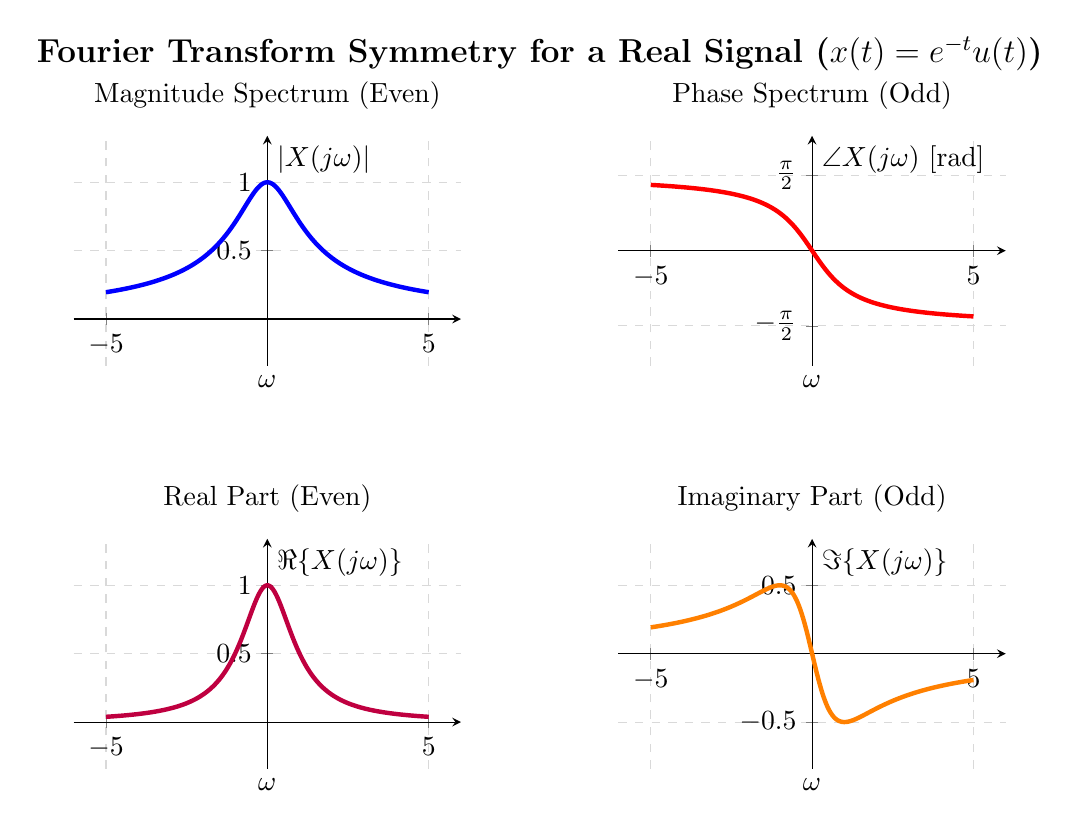
\begin{tikzpicture}
	\begin{groupplot}[
		group style={
			group size=2 by 2,
			horizontal sep=2cm,
			vertical sep=2.2cm, % Slightly increased vertical separation for title space
			group name=my plots,
		},
		width=6.5cm,
		height=4.5cm,
		axis lines=middle,
		enlargelimits=true,
		clip=false,
		xlabel={$\omega$},
		xlabel style={at={(axis description cs:0.5,0)},anchor=north},
		grid=major,
		grid style={dashed, gray!30},
		samples=200,
		domain=-5:5,
		]
		
		% --- PLOT 1: Magnitude Spectrum (Even) ---
		\nextgroupplot[
		title={Magnitude Spectrum (Even)},
		ylabel={$|X(j\omega)|$},
		ytick={0, 0.5, 1},
		ymin=-0.2, ymax=1.2
		]
		\addplot[blue, ultra thick] {1/sqrt(1+x^2)};

		
		% --- PLOT 2: Phase Spectrum (Odd) ---
		\nextgroupplot[
		title={Phase Spectrum (Odd)},
		ylabel={$\angle X(j\omega)$ [rad]},
		ytick={-pi/2, 0, pi/2},
		yticklabels={$-\frac{\pi}{2}$, $0$, $\frac{\pi}{2}$},
		ymin=-2, ymax=2
		]
		% atan returns degrees, convert to radians using rad()
		\addplot[red, ultra thick] {-rad(atan(x))};

		
		% --- PLOT 3: Real Part (Even) ---
		\nextgroupplot[
		title={Real Part (Even)},
		ylabel={$\Re\{X(j\omega)\}$},
		ytick={0, 0.5, 1},
		ymin=-0.2, ymax=1.2
		]
		\addplot[purple, ultra thick] {1/(1+x^2)};

		% --- PLOT 4: Imaginary Part (Odd) ---
		\nextgroupplot[
		title={Imaginary Part (Odd)},
		ylabel={$\Im\{X(j\omega)\}$},
		ytick={-0.5, 0, 0.5},
		ymin=-0.7, ymax=0.7
		]
		\addplot[orange, ultra thick] {-x/(1+x^2)};
	
	\end{groupplot}
	
	% Position the main title centrally above the entire groupplot
	\path (my plots c1r1.north) -- (my plots c2r1.north) 
	node[midway, above=0.7cm, font=\large\bfseries] 
	{Fourier Transform Symmetry for a Real Signal ($x(t) = e^{-t}u(t)$)};
	
\end{tikzpicture}

		\caption{Symmetry properties for real signals: (a) Even magnitude, (b) Odd phase, (c) Even real part, (d) Odd imaginary part}
		\label{fig:symmetry_properties}
	\end{figure}
	
	\section*{12.6 Periodic Signals and Impulse Trains}
	
	\subsection*{12.6.1 Fourier Transform of Periodic Signals}
	
	Periodic signals have Fourier transforms consisting of impulse trains in the frequency domain. This result explains why we can use both Fourier Series and Fourier Transform for periodic signals—they are different representations of the same information.
	
	\begin{theorem}[Fourier Transform of Periodic Signals]
		If $x(t)$ is a periodic signal with period $T_0$ and Fourier series coefficients $a_k$, then:
		\[
		X(j\omega) = 2\pi \sum_{k=-\infty}^{\infty} a_k \delta(\omega - k\omega_0)
		\]
		where $\omega_0 = 2\pi/T_0$ is the fundamental frequency.
	\end{theorem}
	
	\textbf{Proof:} Starting with the Fourier series representation:
	\[
	x(t) = \sum_{k=-\infty}^{\infty} a_k e^{jk\omega_0 t}
	\]
	
	Taking the Fourier transform and using linearity:
	\[
	X(j\omega) = \sum_{k=-\infty}^{\infty} a_k \mathcal{F}\{e^{jk\omega_0 t}\}
	\]
	
	From the frequency shifting property: $e^{jk\omega_0 t} \leftrightarrow 2\pi\delta(\omega - k\omega_0)$
	\[
	X(j\omega) = 2\pi \sum_{k=-\infty}^{\infty} a_k \delta(\omega - k\omega_0)
	\]
	
	\subsection*{12.6.2 Example}
	
	\begin{example}[Impulse Train]
		\textbf{Periodic Impulse Train:} $x(t) = \sum_{n=-\infty}^{\infty} \delta(t - nT_0)$
		
		The Fourier series coefficients are $a_k = 1/T_0$ for all $k$. Therefore:
		\[
		\sum_{n=-\infty}^{\infty} \delta(t - nT_0) \leftrightarrow \frac{2\pi}{T_0} \sum_{k=-\infty}^{\infty} \delta\left(\omega - \frac{2\pi k}{T_0}\right)
		\]
	\end{example}
	
	\subsection*{12.6.3 Relationship Between Fourier Series and Fourier Transform}
	
	The connection between Fourier Series and Fourier Transform for periodic signals is:
	\[
	\text{Fourier Series: } a_k = \frac{1}{T_0} \int_{T_0} x(t)e^{-jk\omega_0 t} \dt
	\]
	\[
	\text{Fourier Transform: } X(j\omega) = 2\pi \sum_{k=-\infty}^{\infty} a_k \delta(\omega - k\omega_0)
	\]
	
	\textbf{Key Insight:} The FT of a CT periodic signal is a weighted impulse train, where:
	\begin{itemize}[noitemsep]
		\item The impulses occur at harmonic frequencies $k\omega_0$
		\item The weight of each impulse is $2\pi a_k$
		\item The spacing between impulses is $\omega_0 = 2\pi/T_0$
	\end{itemize}
	
	\subsection*{12.6.4 Why periodic signals have discrete spectra}
	
	\begin{itemize}[noitemsep]
		\item \textbf{Periodic signals} contain energy only at specific frequencies (harmonics)
		\item \textbf{Impulse trains in frequency} represent this discrete frequency content
		\item \textbf{Dirac delta functions} indicate infinite concentration of energy at specific frequencies
		\item \textbf{Weighted impulses} show the relative strength of each frequency component
	\end{itemize}
	
	\section*{12.7 Convolution and Multiplication Properties}
	
	\subsection*{12.7.1 Convolution Property}
	
	\begin{theorem}[Convolution Property]
		If $x_1(t) \stackrel{\mathcal{F}}{\longleftrightarrow} X_1(j\omega)$ and $x_2(t) \stackrel{\mathcal{F}}{\longleftrightarrow} X_2(j\omega)$, then:
		\[
		x_1(t) \conv x_2(t) \stackrel{\mathcal{F}}{\longleftrightarrow} X_1(j\omega)X_2(j\omega)
		\]
	\end{theorem}
	
	\textbf{Proof:} Let $y(t) = x_1(t) \conv x_2(t) = \int_{-\infty}^{\infty} x_1(\tau)x_2(t-\tau) \dd\tau$. Then:
	\[
	Y(j\omega) = \int_{-\infty}^{\infty} \left[\int_{-\infty}^{\infty} x_1(\tau)x_2(t-\tau) \dd\tau\right] e^{-j\omega t} \dt = X_1(j\omega)X_2(j\omega)
	\]
	
	\textbf{Intuition:} Convolution in time (representing system input-output relationships) becomes simple multiplication in the frequency domain.
	
	\begin{figure}[H]
		\centering
		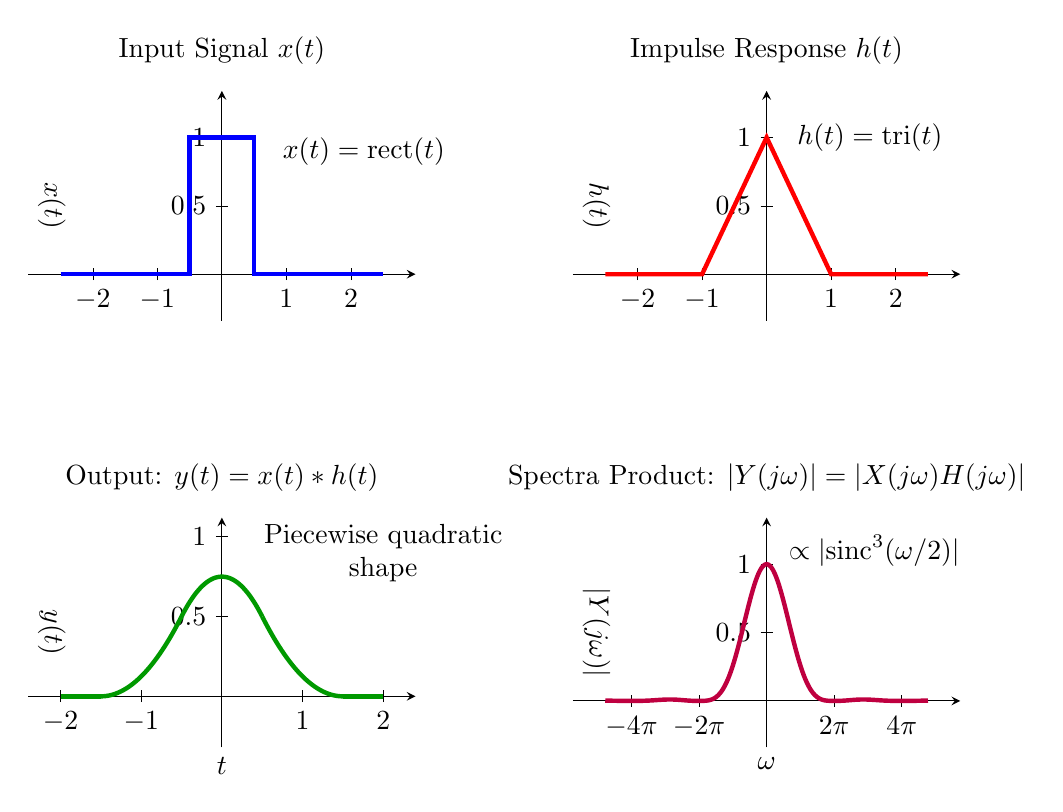
\begin{tikzpicture}
	% Define a common style for all axes for consistency.
	\pgfplotsset{
		myaxes/.style={
			axis lines=middle, enlargelimits=true, clip=false,
			xlabel style={at={(axis description cs:0.5,0)}, anchor=north},
			ylabel style={at={(axis description cs:0,0.5)}, anchor=south, rotate=-90},
			tick style={color=black},
			xtick={-2,-1,0,1,2},
			ytick={0,0.5,1},
			ymin=-0.2, ymax=1.2,
		},
		% Define safe sinc
		/pgf/declare function={
			sinc(\x) = (\x==0) ? 1 : sin(deg(\x))/\x;
		}
	}
	
	\begin{groupplot}[
		group style={
			group size=2 by 2,
			horizontal sep=2cm,
			vertical sep=2.5cm,
			group name=convoplots
		},
		myaxes,
		width=6.5cm,
		height=4.5cm,
		domain=-2.5:2.5,
		samples=201
		]
		
		% --- PLOT 1: Input Signal ---
		\nextgroupplot[title={Input Signal $x(t)$}, ylabel={$x(t)$}]
		\addplot[blue, ultra thick] coordinates {
			(-2.5,0) (-0.5,0) (-0.5,1) (0.5,1) (0.5,0) (2.5,0)
		};
		\node[align=center,fill=white, inner sep=2pt] at (axis cs:2.2,0.9) {$x(t)=\text{rect}(t)$};
		
		% --- PLOT 2: Impulse Response ---
		\nextgroupplot[title={Impulse Response $h(t)$}, ylabel={$h(t)$}]
		\addplot[red, ultra thick] coordinates {
			(-2.5,0) (-1,0) (0,1) (1,0) (2.5,0)
		};
		\node[align=center,fill=white, inner sep=2pt] at (axis cs:1.6,1) {$h(t)=\text{tri}(t)$};
		
		% --- PLOT 3: Convolution Result ---
		\nextgroupplot[
		title={Output: $y(t)=x(t)*h(t)$},
		xlabel={$t$}, ylabel={$y(t)$}, ymax=1.0
		]
		% Piecewise quadratic definition of y(t):
		% y(t) = 0                       for |t| > 1.5
		% y(t) = (t+1.5)^2/2             for -1.5 <= t < -0.5
		% y(t) = 0.75 - t^2/2            for -0.5 <= t < 0.5
		% y(t) = (1.5 - t)^2/2           for 0.5 <= t <= 1.5
		\addplot[green!60!black, ultra thick, domain=-1.5:-0.5] {0.5*(x+1.5)^2};
		\addplot[green!60!black, ultra thick, domain=-0.5:0.5] {0.75 - x^2};
		\addplot[green!60!black, ultra thick, domain=0.5:1.5] {0.5*(1.5 - x)^2};
		\addplot[green!60!black, ultra thick] coordinates {(-2,0) (-1.5,0)};
		\addplot[green!60!black, ultra thick] coordinates {(1.5,0) (2,0)};
	\node[align=center] at (axis cs:2,0.9) {Piecewise quadratic\\shape};
		
		% --- PLOT 4: Multiplication in Frequency Domain ---
		\nextgroupplot[
		title={Spectra Product: $|Y(j\omega)| = |X(j\omega)H(j\omega)|$},
		xlabel={$\omega$}, ylabel={$|Y(j\omega)|$},
		domain=-15:15,
		ytick={0, 0.5, 1},
		xtick={-12.56, -6.28, 0, 6.28, 12.56},
		xticklabels={$-4\pi$, $-2\pi$, $0$, $2\pi$, $4\pi$}
		]
		% Product = sinc^3(ω/2)
		\addplot[purple, ultra thick, smooth] {abs(sinc(x/2)^3)};
		\node[fill=white, inner sep=1pt] at (axis cs:10,1.1)
		{$\propto |\text{sinc}^3(\omega/2)|$};
		
	\end{groupplot}
	
	
\end{tikzpicture}

		\caption{Convolution property: (a) First signal, (b) Second signal, (c) Convolution result, (d) Frequency domain multiplication}
		\label{fig:convolution_property}
	\end{figure}
	
	\subsection*{12.7.2 Multiplication Property}
	
	\begin{theorem}[Multiplication Property]
		If $x_1(t) \stackrel{\mathcal{F}}{\longleftrightarrow} X_1(j\omega)$ and $x_2(t) \stackrel{\mathcal{F}}{\longleftrightarrow} X_2(j\omega)$, then:
		\[
		x_1(t)x_2(t) \stackrel{\mathcal{F}}{\longleftrightarrow} \frac{1}{2\pi}X_1(j\omega) \conv X_2(j\omega)
		\]
	\end{theorem}
	
	\textbf{Intuition:} This is the dual of the convolution property. Multiplication in time corresponds to convolution in frequency, scaled by $1/2\pi$.
	
	\section*{12.8 Examples}
	
	\subsection*{12.8.1 Example 1:}
	
	\begin{example}
		Find the Fourier transform of $x(t) = e^{-a|t|}\cos(\omega_0 t)$ for $a > 0$.
		
		\textbf{Solution:} We can use several properties:
		\begin{enumerate}[noitemsep]
			\item First, note that $\cos(\omega_0 t) = \frac{1}{2}(e^{j\omega_0 t} + e^{-j\omega_0 t})$
			\item From the frequency shifting property: $e^{j\omega_0 t}e^{-a|t|} \leftrightarrow X(j(\omega - \omega_0))$
			\item We know that $e^{-a|t|} \leftrightarrow \frac{2a}{a^2 + \omega^2}$
			\item Using linearity and frequency shifting:
			\[
			e^{-a|t|}\cos(\omega_0 t) \leftrightarrow \frac{a}{a^2 + (\omega - \omega_0)^2} + \frac{a}{a^2 + (\omega + \omega_0)^2}
			\]
		\end{enumerate}
	\end{example}
	
	\subsection*{12.8.2 Example 2:}
	
	\begin{example}
		Find the Fourier transform of $x(t) = \text{rect}(t/2T)$ where $\text{rect}(t) = 1$ for $|t| < 1/2$ and $0$ otherwise.
		
		\textbf{Solution:} Using the time scaling property:
		\begin{enumerate}[noitemsep]
			\item We know that $\text{rect}(t) \leftrightarrow \sinc{\frac{\omega}{2\pi}}$
			\item By time scaling with $a = 1/(2T)$: $\text{rect}(t/2T) \leftrightarrow 2T \sinc{\frac{\omega T}{\pi}}$
		\end{enumerate}
	\end{example}
	
	\section*{12.9 Practice Problems}
	
	\begin{enumerate}[noitemsep]
		\item Find the CTFT of $x(t) = e^{-at}u(t) + e^{at}u(-t)$ for $a > 0$.
		\item Using the differentiation property, find the CTFT of $x(t) = te^{-at}u(t)$.
		\item Show that if $x(t)$ is real and even, then $X(j\omega)$ is real and even.
		\item Find the CTFT of $x(t) = \sin(\omega_0 t)u(t)$.
		\item Using the convolution property, find the CTFT of $x(t) = \text{rect}(t) \conv \text{rect}(t)$.
		\item Find the Fourier transform of the periodic square wave $x(t) = \sum_{n=-\infty}^{\infty} \text{rect}((t-nT)/\tau)$.
		\item Derive the Fourier transform of $x(t) = \cos^2(\omega_0 t)$ using the periodic signals formula.
	\end{enumerate}
	
\section*{12.10 Summary and Next Lecture}
	
	The properties of the CTFT provide a powerful toolkit for signal analysis:
	
	\textbf{Key Properties:}
	\begin{itemize}[noitemsep]
		\item \textbf{Linearity:} Superposition in time $\leftrightarrow$ superposition in frequency
		\item \textbf{Time Shifting:} Delay $\leftrightarrow$ linear phase shift
		\item \textbf{Frequency Shifting:} Modulation $\leftrightarrow$ spectrum translation
		\item \textbf{Time Scaling:} Time compression $\leftrightarrow$ frequency expansion
		\item \textbf{Differentiation:} Time derivative $\leftrightarrow$ multiplication by $j\omega$
		\item \textbf{Integration:} Time integral $\leftrightarrow$ division by $j\omega$
		\item \textbf{Convolution:} Time convolution $\leftrightarrow$ frequency multiplication
		\item \textbf{Symmetry:} Real signals have conjugate symmetric spectra
		\item \textbf{Periodic Signals:} Periodic signals have impulse train spectra
		\item \textbf{Next time:} Convolution property and LTI analysis in the frequency domain
	\end{itemize}
\end{document}
